\documentclass{beamer}

%Document language and encoding
\usepackage[english]{babel}
\usepackage[utf8]{inputenc}
\usepackage[T1]{fontenc}
\selectlanguage{english}
\usepackage{array}
\usepackage{tabularx}
\usepackage{tabulary}
\usepackage{multirow}
\usepackage{booktabs}
%\setbeamertemplate{caption}[numbered]
\usepackage{caption}
\usepackage{siunitx} \sisetup{load-configurations=abbreviations} %use correctly typed SI units
\usepackage{xspace}
\captionsetup[figure]{labelformat=empty}
\newcommand{\figh}[1]{\includegraphics[width=0.4\linewidth]{#1}}
\newcommand{\figv}[1]{\includegraphics[height=0.15\textheight,keepaspectratio]{#1}}
\newcolumntype{P}[1]{>{\centering\arraybackslash}p{#1}}
\hypersetup
{
        colorlinks=false,
        linkcolor=black,       % \ref{...} and \pageref{...}
        urlcolor=black,       % \href{...}{...} external (URL)
        filecolor=black,     % \href{...} local file
        pdftitle={ET4171 Processor Design Project},
        pdfauthor={Henrique Dantas and Luca Feltrin},
        pdfsubject={LEON3 processor optimization},
        pdfkeywords={},
        pdfproducer={pdfLaTeX},
        bookmarksopen=true,
        pdfborder={0 0 0}
}


\usetheme[pageofpages=of,% String used between the current page and the
                         % total page count.
          %bullet=circle,% Use circles instead of squares for bullets.
          titleline=true,% Show a line below the frame title.
          alternativetitlepage=true,% Use the fancy title page.
          titlepagelogo=Figures/tudelft,% Logo for the first page.
          %watermark=watermark-polito,% Watermark used in every page.
          %watermarkheight=100px,% Height of the watermark.
          %watermarkheightmult=4,% The watermark image is 4 times bigger
                                % than watermarkheight.
          ]{Torino}
%\usecolortheme{nouvelle}

\newenvironment<>{newblock}[1]{%
    \begin{actionenv}#2%
        \def\insertblocktitle{#1}%
        \par%
        \mode<presentation>{%
            \setbeamercolor{block title}{fg=white,bg=chameleongreen3}
            \setbeamercolor{block body}{fg=black,bg=white}
            \setbeamercolor{itemize item}{fg=green!20!black}
            \setbeamercolor{itemize subitem}{fg=green}
            %\setbeamertemplate{itemize item}[+]
        }%
    \usebeamertemplate{block begin}}{\par\usebeamertemplate{block end}\end{actionenv}
}

\definecolor{pbgray}{RGB}{51,149,48}% background color for the progress bar
\definecolor{chameleongreen1}{RGB}{98,189,25}
\definecolor{chameleongreen2}{RGB}{188,225,141}
\definecolor{chameleongreen3}{RGB}{51,149,48}
\definecolor{chameleongreen4}{RGB}{0,98,90}


\newenvironment<>{problock}[1]{%
    \begin{actionenv}#2%
        \def\insertblocktitle{#1}%
        \par%
        \mode<presentation>{%
            \setbeamercolor{block title}{fg=white,bg=green!20!black}
            \setbeamercolor{block body}{fg=black,bg=green!10!black!10}
            \setbeamercolor{itemize item}{fg=green!20!black}
            \setbeamercolor{itemize subitem}{fg=green}
            %\setbeamertemplate{itemize item}[+]
        }%
    \usebeamertemplate{block begin}}{\par\usebeamertemplate{block end}\end{actionenv}
}

\newenvironment<>{conblock}[1]{%
    \begin{actionenv}#2%
        \def\insertblocktitle{#1}%
        \par%
        \mode<presentation>{%
            \setbeamercolor{block title}{fg=white,bg=red!40!black}
            \setbeamercolor{block body}{fg=black,bg=red!10}
            \setbeamercolor{itemize item}{fg=red!40!black}
            \setbeamercolor{itemize subitem}{fg=red}
            %\setbeamertemplate{itemize item}[-]
        }%
    \usebeamertemplate{block begin}}{\par\usebeamertemplate{block end}\end{actionenv}
}


\usepackage{tikz}
\usetikzlibrary{calc}



%% ORIGINAL COLOR %% \definecolor{pbgray}{HTML}{575757}% background color for the progress bar
\makeatletter
\def\progressbar@progressbar{} % the progress bar
\newcount\progressbar@tmpcounta% auxiliary counter
\newcount\progressbar@tmpcountb% auxiliary counter
\newdimen\progressbar@pbht %progressbar height
\newdimen\progressbar@pbwd %progressbar width
\newdimen\progressbar@tmpdim % auxiliary dimension

\progressbar@pbwd=\textwidth
\progressbar@pbht=0.5pt
%%http://tex.stackexchange.com/questions/59742/progress-bar-for-latex-beamer
% the progress bar
\def\progressbar@progressbar{%

    \progressbar@tmpcounta=\insertframenumber
    \progressbar@tmpcountb=\inserttotalframenumber
    \progressbar@tmpdim=\progressbar@pbwd
    \advance\progressbar@tmpcountb by -2
    \advance\progressbar@tmpcounta by -2
    \multiply\progressbar@tmpdim by \progressbar@tmpcounta
    \divide\progressbar@tmpdim by \progressbar@tmpcountb

  \begin{tikzpicture}[very thin]
    \draw[chameleongreen3!60,line width=\progressbar@pbht] (0pt,0pt) -- ++ (\progressbar@pbwd,0pt);
    \draw[draw=none]  (\progressbar@pbwd,0pt) -- ++ (2pt,0pt);

    \draw[fill=pbgray!60,draw=none] %
       ( $ (\progressbar@tmpdim, \progressbar@pbht) + (0,-3.5pt) $ ) -- ++(60:6pt) -- ++(180:6pt) -- ++ (300:6pt) ;

   % \node[draw=pbgray!30,text width=3.5em,align=center,inner sep=1pt,
   %  text=pbgray!70,anchor=east] at (0,0) {\insertframenumber/\inserttotalframenumber};
  \end{tikzpicture}%
}

\addtobeamertemplate{headline}{}
{%
  \begin{beamercolorbox}[wd=\paperwidth,ht=-1.5ex,center,dp=1ex]{white}%
    \progressbar@progressbar%
  \end{beamercolorbox}%
}
\makeatother



\begin{document}

\title{\textbf{ET4171 Processor Design Project}}
\subtitle{LEON3 processor optimization }
\author{Henrique~Dantas\\
\vspace{0.5cm} Luca~Feltrin}
\institute{Delft University of Technology}
\date{\today} 

{ % to delimit a block (we only want to remove the header for this frame)
\makeatletter % to change template
    \setbeamertemplate{headline}[default] % not mandatory, but I though it was better to set it blank
    \def\beamer@entrycode{\vspace*{-\headheight}} % here is the part we are interested in :)
\makeatother
\frame{\titlepage}
}

\renewcommand{\arraystretch}{1.3}
\newcommand{\dollar}{\$}
\renewcommand{\kHz}{\si{\kHz}\xspace}
\renewcommand{\MHz}{\si{\MHz}\xspace}
\renewcommand{\W}{\si{\W}\xspace}
\renewcommand{\s}{\si{\s}\xspace}
\newcommand{\Oppers}{~\si[per-mode=symbol]{Op\per\s}\xspace}

\frame{\frametitle{Table of contents}\tableofcontents} 

\section{Objectives}
%\addtocounter{section}{1}


\frame{\frametitle{Objectives}
\begin{itemize}
\item Target: Embedded applications 
\begin{itemize} \item Compound metric: \texttt{P$\times$BS} \end{itemize}
\item Poor Mul/Div execution time
\begin{itemize} \item Implementation with different algorithms \end{itemize}
\end{itemize}
}

\section{Multiplier}
\frame{\frametitle{Multiplier: Wallace Tree}
Algorithm:
\begin{enumerate}
\item Initial \texttt{AND}ing between inputs.
\item Reduce tree using Full Adders and Half Adders.
\item Add the two remaining numbers with a traditional adder.
\end{enumerate}
}

\frame{\frametitle{Pros and Cons}
\begin{columns}
\begin{column}{0.40\textwidth}
\begin{problock}{Pros}
\begin{itemize}
\item Speed improvement.
\item Regular structure.
\end{itemize}
\end{problock}
\end{column}

\begin{column}{0.45\textwidth}
\begin{conblock}{Cons}
\begin{itemize}
\item Resource usage is high.
\item Signifcant Area footprint.
\item Increase in power.
\end{itemize}
\end{conblock}
\end{column}
\end{columns}
}

\frame{\frametitle{Implementation Details}
3 Input Signals:\texttt{RST}, \texttt{CLK} and \texttt{MULI}\\
1 Output Signal:\texttt{MULO}\\
4 generics: \texttt{infer}, \texttt{multype}, \texttt{pipe} and \texttt{mac}

Constants used: WallaceTree (3D logic vector), stages, FA, HA, CIN and RE.
}

\frame{\frametitle{Implementation Details II}
For negative operation - Alternative Baugh Wooley
Negate AND operations (when includes MSD from op1 or op2 but not both)
Add a constant vector at the end.
}

\frame{\frametitle{Implementation Details III}
Feed inputs to FOR-GENERATES (with IF-GENERATES)
IF holdn is HIGH update Add the two final numbers with Baugh-Wooley vector (for signed operations) (ready and nready are not used).
Update MULO.(result/ICC).
}

\section{Divider}
\frame{\frametitle{Divider: Which algorithm?}
\begin{table}
\centering
\begin{tabular}{lcc}
Repeated Multiplication	& \color{green!50!black} \bfseries Fast	& \color{red!40!black} \bfseries Area\\
Reciprocation			& \color{green!50!black} \bfseries Fast	& \color{red!40!black} \bfseries Area\\
Array Divider			& \multicolumn{2}{c}{\color{red!40!black} \bfseries No control on physical placing}\\
Radix >8				& \color{green!50!black} \bfseries Fast	& \color{red!40!black} \bfseries Area\\
Radix-4					& \multicolumn{2}{c}{\color{green!50!black} \bfseries Good compromise}\\
\end{tabular}
\end{table}
\vspace{0.5cm}
\begin{center}
\large \bfseries Execution time $\approx \frac{1}{2}$ of the baseline
\end{center}
}

\frame{\frametitle{Divider II}
\begin{figure}
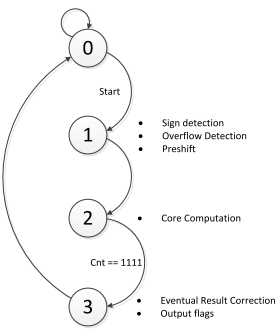
\includegraphics[width=0.9\textwidth,height=0.8\textheight,keepaspectratio]{Figures/DivisorStateMachine.png}
\caption{}
\end{figure}
}

\frame{\frametitle{Divider III}
\begin{figure}
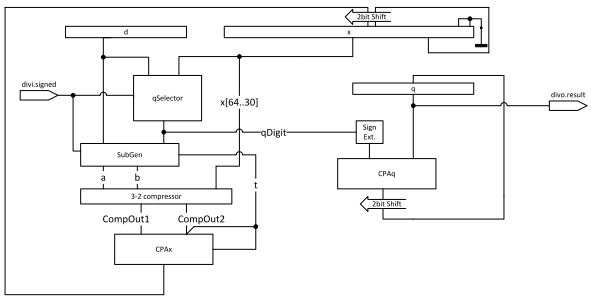
\includegraphics[width=0.9\textwidth,height=0.8\textheight,keepaspectratio]{Figures/DivisorDiagram.png}
\caption{}
\end{figure}
}

\frame{\frametitle{Dvider IV}
\begin{itemize}
\item Signed division (signed p-d plot) vs. Unsigned division (half p-d plot) + 1 cycle for sign
\begin{itemize}
\item No area differences but 1 more cycle delay: signed Division
\end{itemize}
\end{itemize}
}

\frame{\frametitle{Divider V}
\begin{figure}
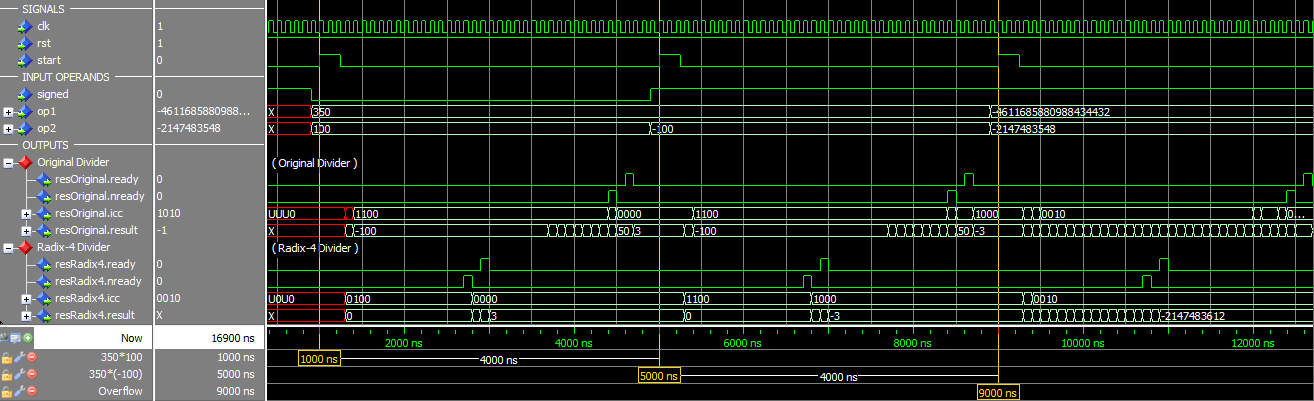
\includegraphics[width=0.9\textwidth,height=0.8\textheight,keepaspectratio]{Figures/myDivisionvsOriginal.png}
\caption{Baseline vs. Radix-4: 19 cycles vs 36}
\end{figure}
}

\section{Synthesis Results}
\frame{\frametitle{Synthesis Results}

\begin{table}[H]
\centering
\begin{tabular}{cccc}
& Baseline & Div & Div\&Mul\\
\midrule
Clock freq. [\MHz]) & 80.522 & 80.535 & 40.197\\
Slices & 9904 & 10479 & 11886\\
LUTs & 16889 & 17865 & 20469\\
Quiescent power [\W] & 2.467 & 2.468 & 2.511\\
Dynamic power [\W] & 0.721 & 0.743 & 0.832\\
Total power [\W] & 3.188 & 3.211 & 3.343\\
P/f [\si[per-mode=symbol]{\W\per\MHz} ] & 0.03959 & 0.03987 & 0.08317\\\toprule
\end{tabular}
\end{table}
}


\section{Benchmarks Scores}
\frame{\frametitle{Benchmarks Scores}
%\fontsize{10pt}{8}\selectfont
\vspace{-.5cm}
\begin{table}[H]
\centering
\begin{tabular}{ccc}
& Baseline & Modified\\
\midrule
Stanford [\s] & 2.30 & 2.21\\
Whetstone [\s] & 116.2 & 112.08\\
Gmpbench Multiply [\Oppers] & 781 & 914\\
Gmpbench Divide [\Oppers] & 15876 & 19205\\
Gmpbench RSA [\Oppers] & 5123 & 5353\\
Division [\s] & 8.06 & 7.31\\
Mibench JPEG (average) [\s] & 23.215 & 21.76\\
SSD [\s] & 10.59 & 8.60\\
Total [\s] & \textbf{219.28} & \textbf{206.92}\\
\toprule
\end{tabular}
\end{table}
%Only slight improvement probably due to the Operating System's Scheduling
}

\section{Conclusion}
\frame{\frametitle{Conclusion - Comparison with Matrics (Div)}

\begin{table}[H]
\centering
\begin{tabular}{cccc}
&Baseline & Modified & Improvements\\\midrule
\ttfamily A & 2.68 & 2.83 & \color{red!40!black} -5.8\%\\
\ttfamily D & 1.24 & 1.24 & - \\
\ttfamily P & 3.19 & 3.21 & \color{red!40!black} -0.7\%\\
\ttfamily BS & 2.19 & 2.13 & \color{green!40!black} 2.7\%\\\midrule
\ttfamily A$\times$D & 3.33 & 3.52 & \color{red!40!black} -5.8\%\\
\ttfamily A$\times$BS & 5.88 & 6.05 & \color{red!40!black} -2.9\%\\
\ttfamily P$\times$D & 3.96 & 3.99 & \color{red!40!black} -0.7\%\\
\ttfamily P$\times$BS & 6.69 & 6.85 & \color{green!40!black} 2.08\%\\
\end{tabular}
\end{table}
}

\frame{\frametitle{Conclusion II - Comparison with Matrics (Div \& Mul)}
\begin{table}[H]
\centering
\begin{tabular}{cccc}
&Baseline & Modified & Improvements\\\midrule
\ttfamily A & 2.68 & 3.24 & \color{red!40!black} -21\%\\
\ttfamily D & 1.24 & 2.49 & \color{red!40!black} -100\%\\
\ttfamily P & 3.19 & 3.34 & \color{red!40!black} -5.0\%\\
\ttfamily BS & 2.19 & 2.07 & \color{green!40!black} 6\%\\\midrule
\ttfamily A$\times$D & 3.33 & 8.05 & \color{red!40!black} -142\%\\
\ttfamily A$\times$BS & 5.88 & 6.69 & \color{red!40!black} -14\%\\
\ttfamily P$\times$D & 3.96 & 8.32 & \color{red!40!black} -100\%\\
\ttfamily P$\times$BS & 6.69 & 6.92 & \color{green!40!black} 1\%\\
\end{tabular}
\end{table}
}

\section{Further Improvements}
\frame{\frametitle{Further Improvements}
\begin{itemize} \item Cache size
	\begin{itemize} \item More power consumption, need to determine actual miss rate
	\end{itemize}

\item Branch prediction
	\begin{itemize} \item Now: Static prediction, only slight advantage, power consumption
	\end{itemize}
	
 \item Out of Order Execution
	\begin{itemize} \item Radical change of the integer unit, improved execution time
	\end{itemize}
	\end{itemize}
}

\end{document}
